%----------------------------------------------------------------------------------------
%	PACKAGES AND DOCUMENT CONFIGURATIONS
%----------------------------------------------------------------------------------------

\documentclass[12pt,a4paper]{article}

\usepackage[version=3]{mhchem} % Package for chemical equation typesetting
\usepackage{siunitx} % Provides the \SI{}{} and \si{} command for typesetting SI units
\usepackage{graphicx} % Required for the inclusion of images
\usepackage{natbib} % Required to change bibliography style to APA
\usepackage{amsmath} % Required for some math elements 
\usepackage{geometry}
\usepackage{enumerate}
\usepackage{float}
\usepackage{subfigure}
\usepackage{pdfpages}
\usepackage{siunitx}
\usepackage{fancyhdr}
\usepackage{textcomp}

\includepdfset{pagecommand={\thispagestyle{fancy}}}%page number for pdf

\renewcommand{\labelenumi}{\alph{enumi}.} % Make numbering in the enumerate environment by letter rather than number (e.g. section 6)
\geometry{left=2cm,right=2cm,top=3cm,bottom=3cm}

%\usepackage{times} % Uncomment to use the Times New Roman font

%----------------------------------------------------------------------------------------
%	DOCUMENT INFORMATION
%----------------------------------------------------------------------------------------


\begin{document}

\begin{center}
~\\
\rule[0mm]{400pt}{0.5pt}
\Large{ \textsc{\newline\\UM-SJTU Joint Institute\\Physics Laboratory\\(Vp141)\\}}
\rule[0mm]{400pt}{0.5pt}
\Large{ \textsc{\newline\newline\newline\newline\newline\newline\\
Laboratory Report\\}}
\Large{\textsc{ \\ Exercise 4  \\ The sound velocity} }

\end{center}

\begin{description}
    \item[] 
    \item[] 
    \item[] 
    \item[] 
    \item[] 
    \item[]
    \item[]\qquad \qquad Name: Han Yibei \qquad ID:519370910123   \qquad    Group:11\\
    \item[]\qquad \qquad Date: \today
\end{description}

\newpage

%----------------------------------------------------------------------------------------
%	SECTION 1
%----------------------------------------------------------------------------------------

\section{Introduction}

The objective of this experiment is to use three methods to measure the speed of the sound in air: the resonance method, the phase comparison method and the time difference method. The methods of operating a function generator and an oscilloscope are also studied.

\section{Theoratical background}
\subsection{Basic Quantitative Characteristics of Sound Waves}

Sound is a longitudinal wave propagating through a compressible medium as the direction of the medium vibrations is the same as that of propagation. The frequency of sound perceptible to human ears is within the range of 20Hz to 20000Hz. In this experiment, we use ultrasonic wave because its wavelength is short enough to be measured in a teaching lab.\par 
The formula of the phase speed $v$, the frequency $f$, and the wavelength $\lambda$ is
\begin{equation}
    v=\lambda f
\end{equation}\par 
For motion with constant speed $v$ along a straight line with distance $L$ over time $t$, we have:
\begin{equation}
    v=\frac{L}{t}
\end{equation}

\subsection{Measurement Method}
\subsubsection{Resonance Method}

The distance between the wave source(s1) and the receiver(s2) is $L$. when arranged parallel to each other, the sound wave will be reflected. If $L$ satisfies:
\begin{equation}
    L=n \frac{\lambda}{2} 
    \Longrightarrow 
    \lambda=\frac{2L}{n}
\end{equation}                     
Where n=1, 2,…. , standing waves will form as the distance is a multiple of half of the wavelength. Under this circumstance, a maximum output power will be observed in the oscillography. As shown in figure 1, the interval between two maximum points is $\lambda/2$. Therefore, $\lambda$ can be measured from the oscillography. By reading the frequency $f$ from the signal generator, we can calculate the wavelength using Eq.1. 

\begin{figure}[H]
    \centering
    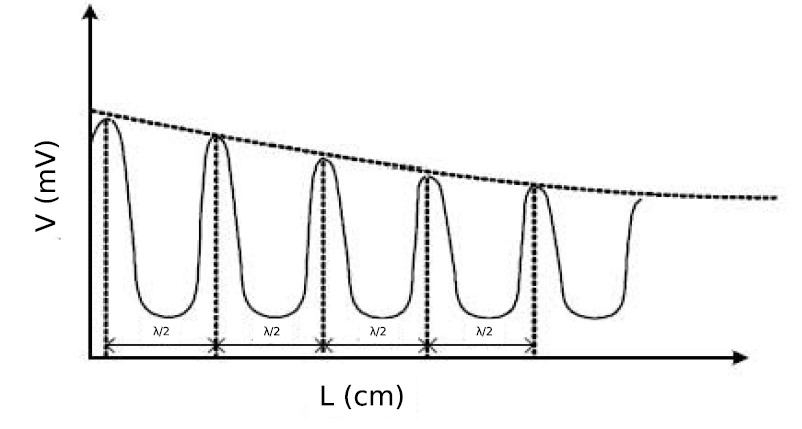
\includegraphics[width=10cm]{resonance.jpg}
    \caption{Relationship between the signal voltage and the distance between the transducers}
\end{figure}

\subsubsection{Phase-comparison Method}
Lissajous figures are used to display the trajectories of a particle moving simultaneously in two perpendicular directions. On x direction the wave function is $A_xcos⁡(\omega_xt+\varphi_x)$ and on y direction the wave function is $A_y cos⁡(\omega_yt+\varphi_y)$. Therefore, the trajectory of the particle is $r(t)=(A_xcos⁡(\omega_xt+\varphi_x),A_ycos⁡(\omega_y t+\varphi_y))$. When the two superimposed harmonic motions have identical frequency $\omega_x=\omega_y$ and $|\varphi_x-\varphi_y|=n\pi (n=0,1,2…)$, the Lissajous figure will show a straight line. For other phase difference values the figure will show corresponding elliptical shapes. \par 
\begin{equation}
    L=n\lambda \Longrightarrow \lambda=\frac{L}{n}
\end{equation}
In this experiment, we find different values of $L$ when a line of the same slope is displayed. When the distance increases by $\lambda$, $\varphi$ increases by 2$\pi$, and the superimpose figure can be the same. Therefore, the slope of the linear fit of $L$ v.s. $i$ is $\lambda$. 

\subsubsection{Time-difference Method}
When S2 receives an ultrasonic pulse signal emitted by S1, one can measure the time interval for the sound travelling from S1 to S2. When $L$ and $t$ is known, the speed of sound can be calculated from Eq.2.

\section{Apparatus}
Shown in figure 2 are the components of the transducer and oscilloscope.
\begin{figure}[H]
    \centering
    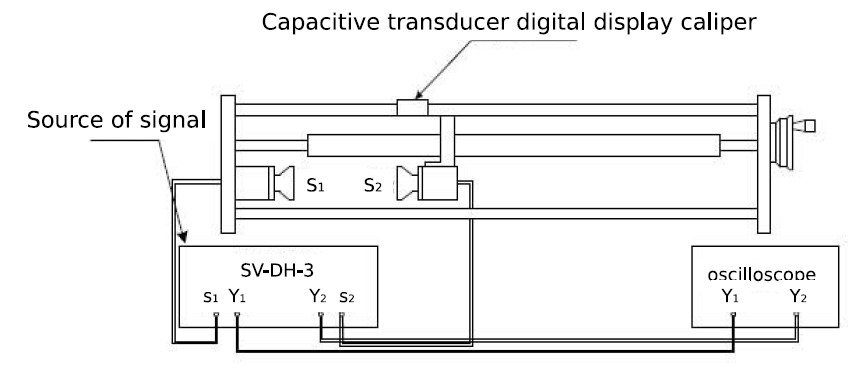
\includegraphics[width=10cm]{setup.jpg}
    \caption{Experimental Setup}
\end{figure}

The information of each measurement device is shown in Table 1.

\begin{table}[H]
    \centering
    \begin{tabular}{|c|c|c|c|c|}
        \hline
        Apparatus &Measurements & Range & Minimum scale & Apparatus uncertainty\\
        \hline
        Thermometer & temperature &  -10-50\textcelsius & 1\textcelsius & $\pm$1\textcelsius\\  
        \hline
        Signal generator & frequency& / & 0.001kHz & $\pm$ 0.001kHz\\
        \hline
        Scale on the transducer & length & 0-300mm & 0.001mm	& $\pm$ 0.001mm\\
        \hline
        Cursor function & time & / & 0.2$\mu s$ & $\pm$0.2$\mu s$ \\
        \hline
    \end{tabular}
    \caption{Information of Each Measurement Device}
\end{table}
 
\section{Measurement}
\subsection{Resonance Method}
\begin{enumerate}
    \item First set the distance between S1 and S2 at about 10mm.
    \item  Device Initialization: Turn on the signal source and the oscilloscope. Then set the Method on the signal source to be continuous. Adjust Signal Strength until a 10V peak is displayed on the oscilloscope. Adjust signal frequency between 34.5 kHz and 40 kHz until the peak-to-peak voltage reaches its maximum. Record the frequency.
    \item Move S2 away from S1 to increase L and observe the figure shown on the oscilloscope. Record the position of S2 when the output voltage reaches its maximum.
    \item Repeat step 3 to record 12 values of L and apply linear fit to get the value of v.
\end{enumerate}

\subsection{Phase-comparison Method}
\begin{enumerate}
    \item Set the device to corresponding mode. 
    \item Increase the distance and record the distance when there is a straight up-right line shown on the screen.
    \item Repeat step 2 and collect 12 sets of data in total.
    \item Apply linear fit to get the value of v.
\end{enumerate}

\subsection{Time difference Method} 
\begin{enumerate}
    \item Set the device to corresponding mode. The frequency of the source set to 100Hz and the width set to 500µs. Set the initial distance to be larger than 100mm.
    \item Set the distance to be different values and record the time the wave needs to propagate.
    \item Collect 12 sets of data and apply linear fit to get the value of v.
\end{enumerate}

\section{Result}
\subsection{Initial settings}
The temperature is measured at 26$\pm$1\textcelsius.\par 
The frequency we choose is 38.561$\pm$0.001kHz=38561$\pm$1Hz.

\subsection{Resonance Method}
According to Eq.3, we want to know the value of $\lambda$, so we apply linear fit of L v.s. I, shown in figure3. All the measurement data are listed in appendix B.
\begin{figure}[h]
    \centering
    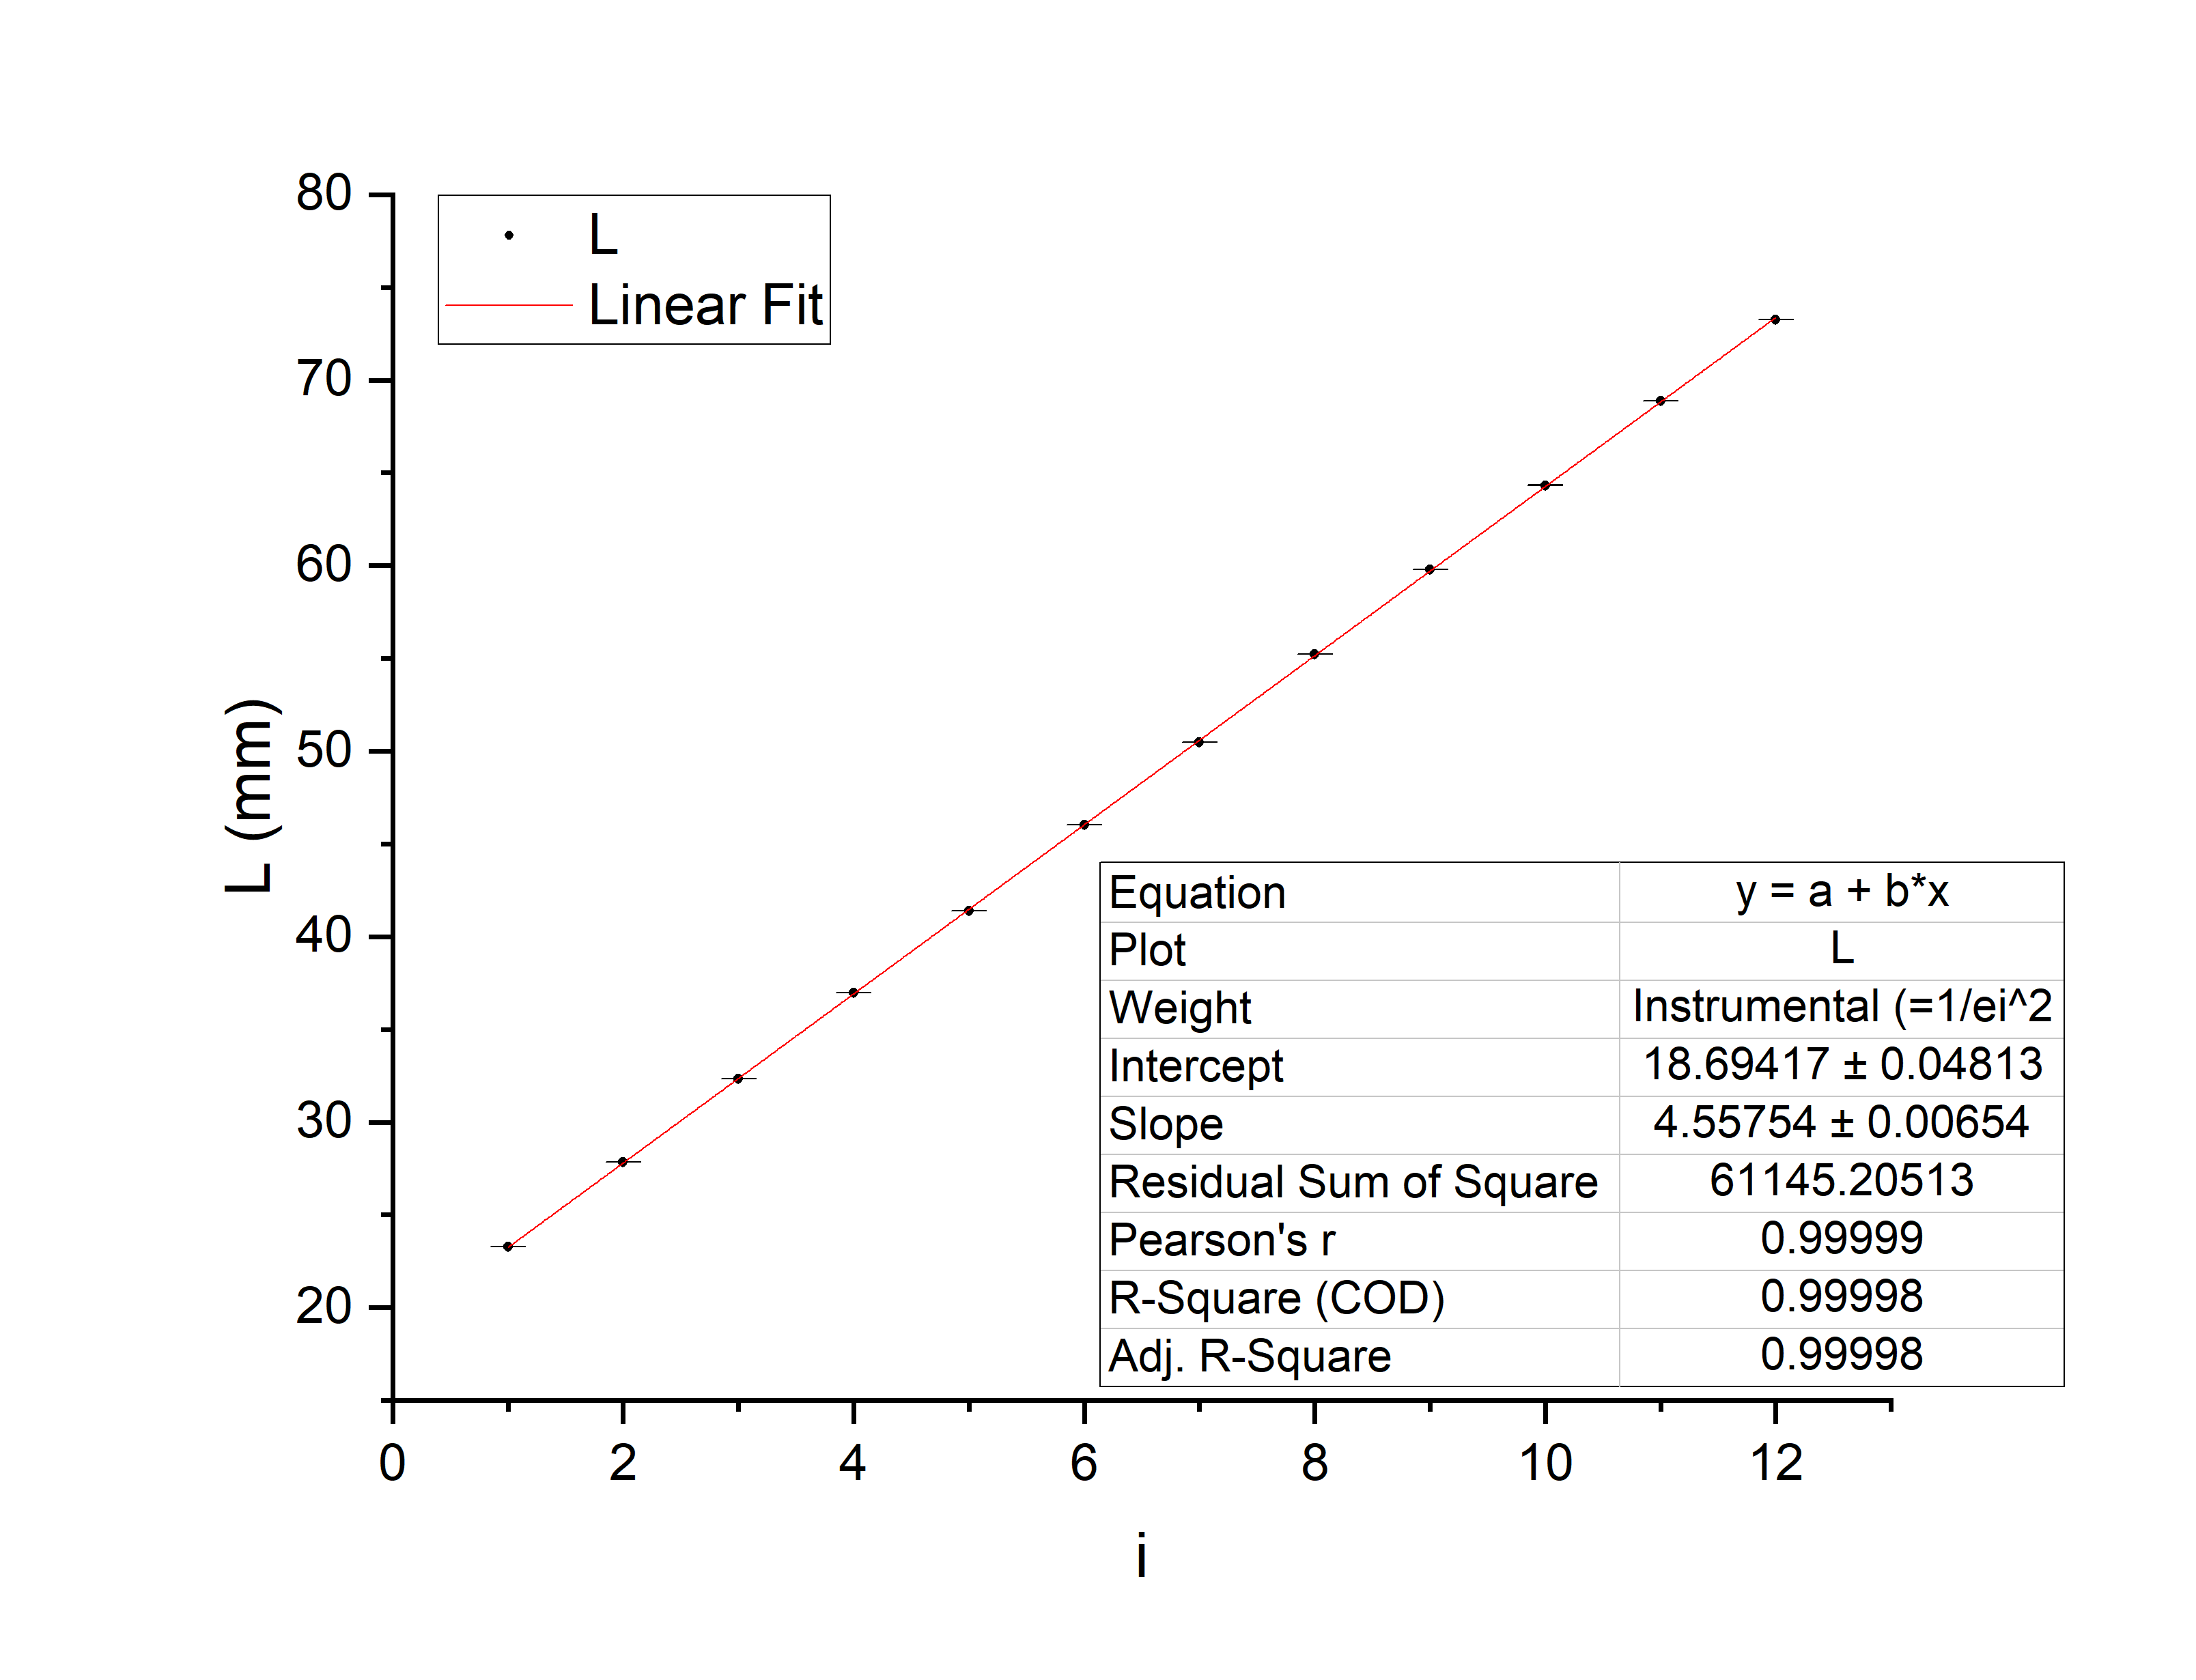
\includegraphics[width=10cm]{method1.png}
    \caption{Linear fit of L v.s. i}
\end{figure} \par
Obtained from the figure, the slope is 4.55754mm and the standard error is 0.00654mm. The CI  half-width is $0.00654\times t_{12,0.95}=0.00654\times 2.179=0.01425066mm$, rounded to be $0.014mm$. Therefore, the uncertainty of the slope is $0.014mm$. Since the slope equals  $\frac{\lambda}{2}$, we obtain the rounded $\lambda =2\times 4.55754 mm=9.12\pm 0.03 mm=9.12\times 10^{-3}\pm 0.03\times 10^{-3}m$. According to Eq.1, $v=\lambda f=9.12\times 10^{-3}\times 38561=351.5\pm 1.1m/s$. Since the R-square obtained is bigger than 0.75, the linear is well fit.

\subsection{Phase-comparison Method}
\begin{figure}[H]
    \centering
    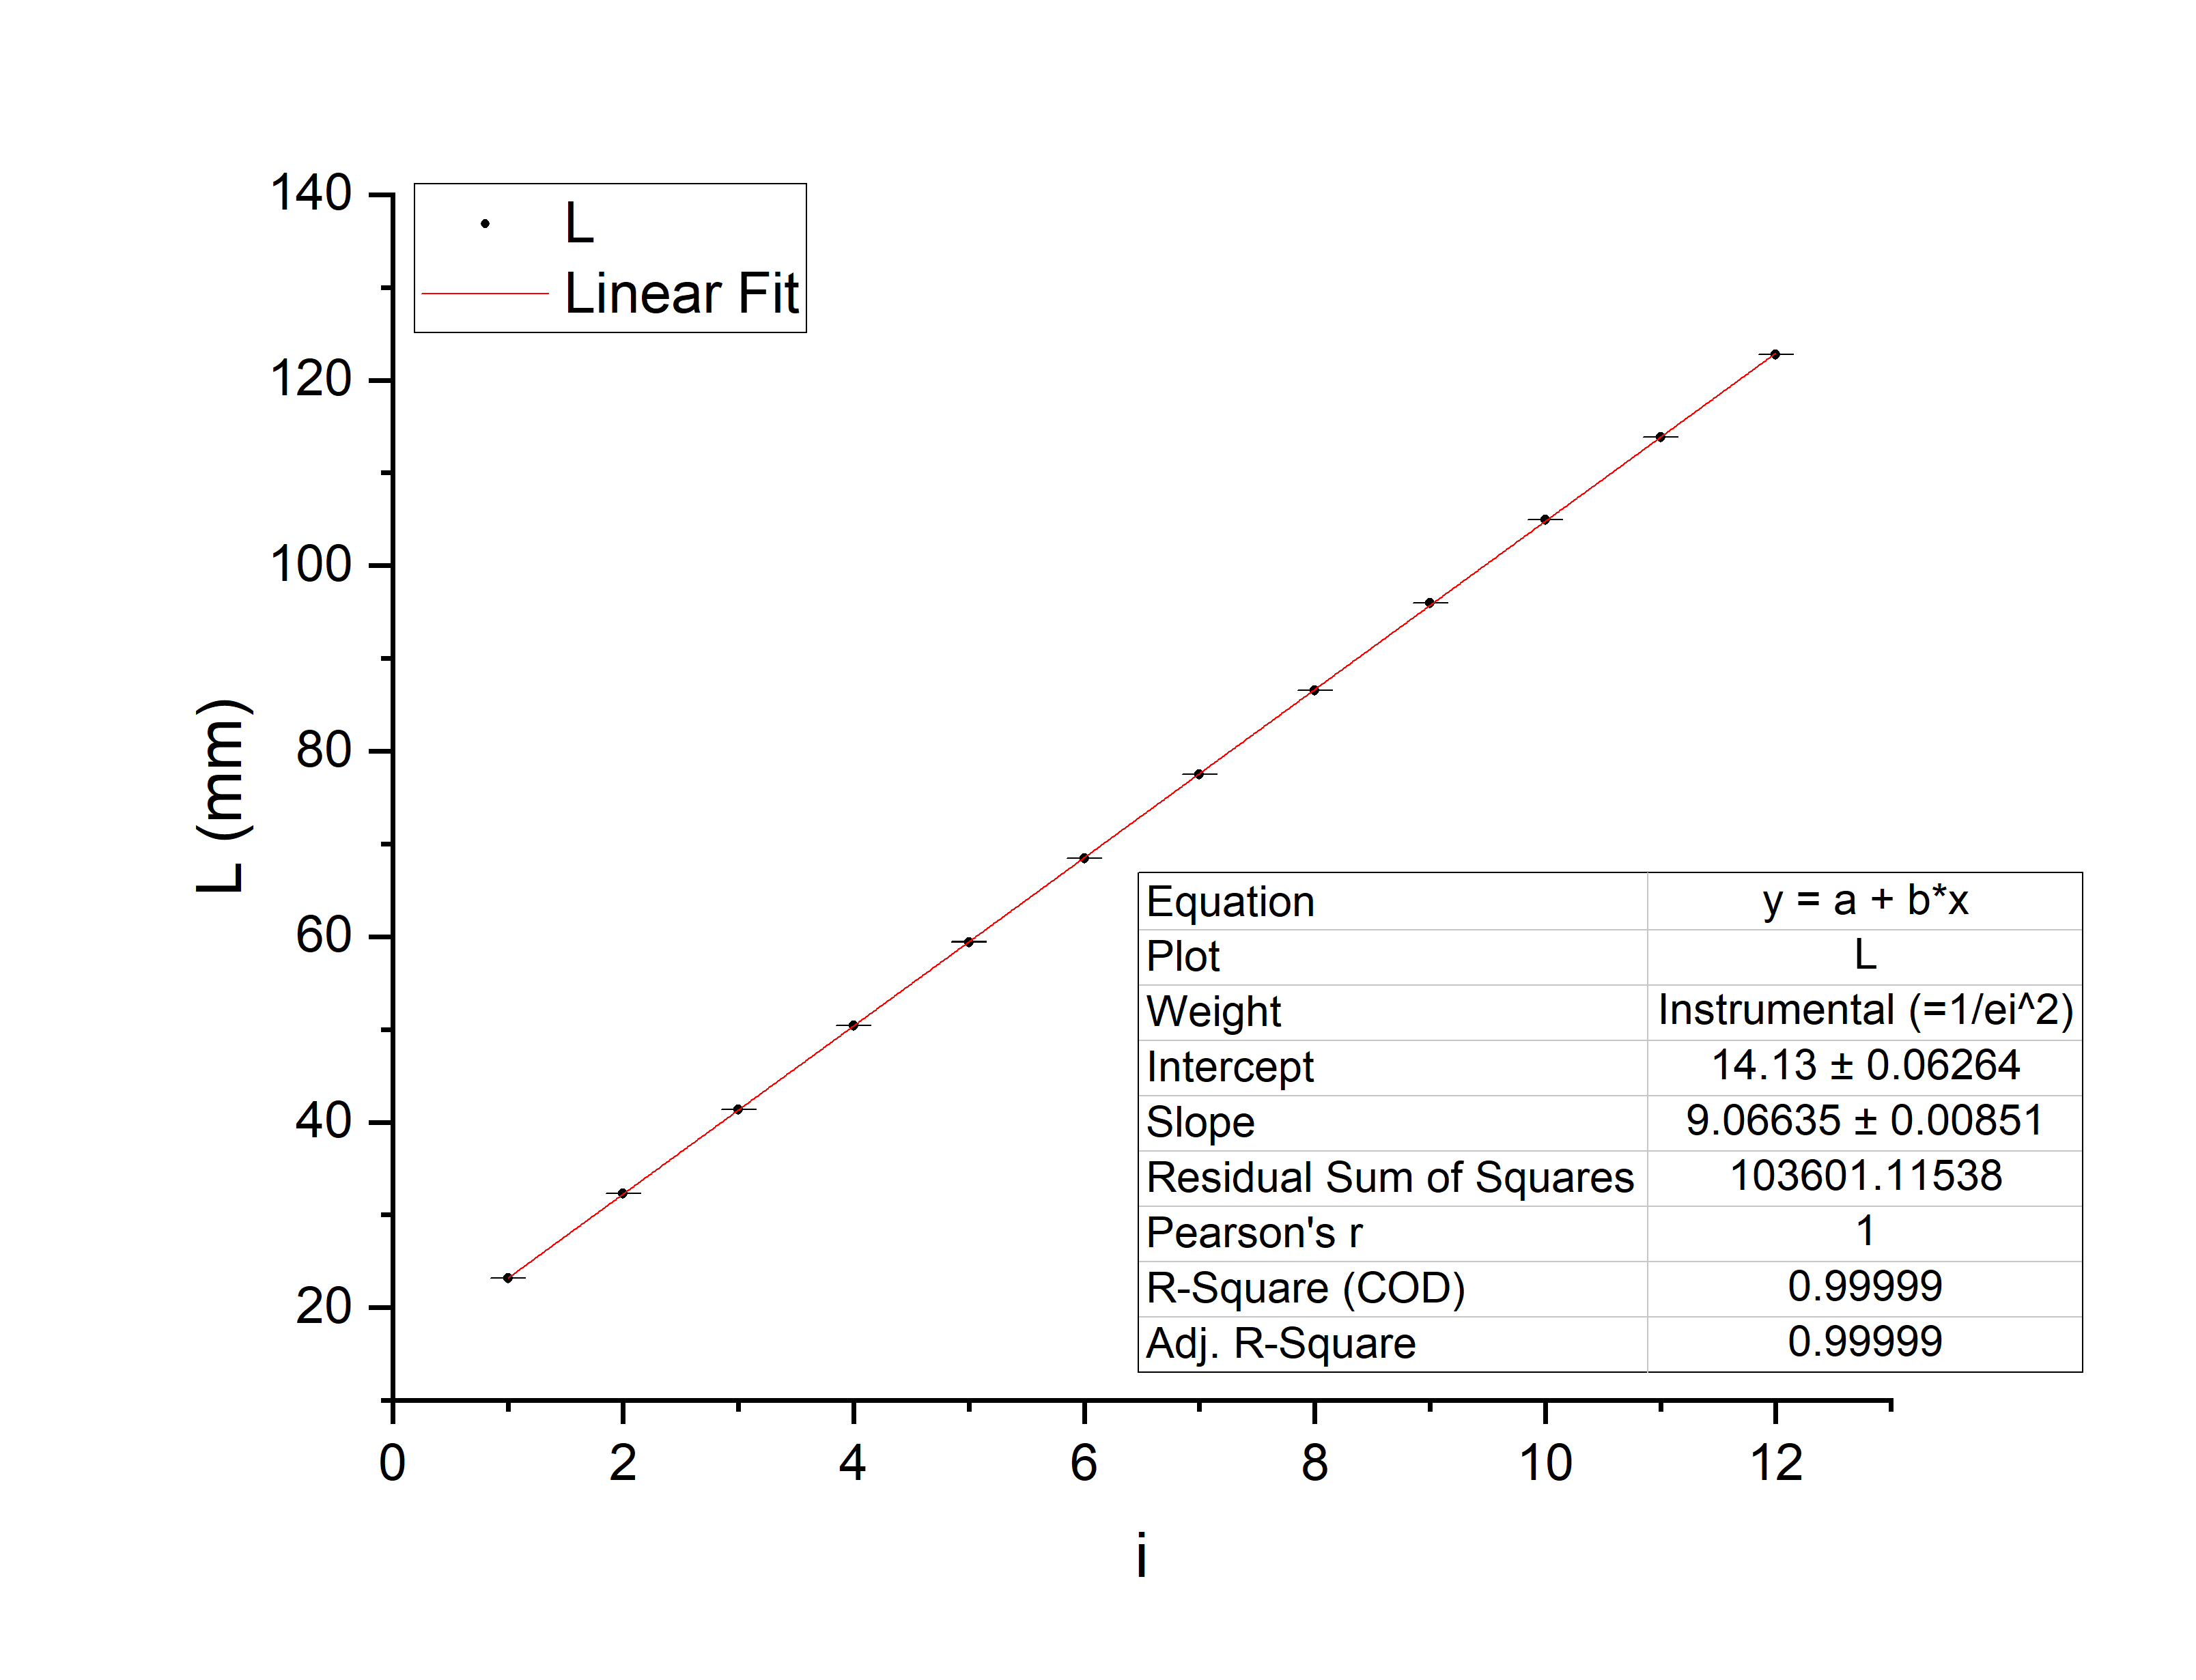
\includegraphics[width=10cm]{method2.png}
    \caption{Linear fit of L v.s. i}
\end{figure} \par
Obtained from the figure, the slope is 9.06635mm and the standard error is 0.00851mm. The CI half-width is $0.00851\times t_{12,0.95}=0.00851\times2.179=0.01854329\mu s/mm$, rounded to be $0.019 \mu s/mm$. Therefore, the uncertainty of the slope is $0.019\mu s /mm$. Since the slope equals $\lambda$, we obtain the rounded $λ=9.066\pm 0.019 mm=9.066\times 10^{-3}\pm 0.019\times 10^{-3} m$.
According to Eq.1, $v=\lambda f=9.066\times 10^{-3}\times 38561=349.6\pm 0.7m/s$. Since the R-square obtained is bigger than 0.75, the linear is well fit.

\subsection{Time Difference Method}
As t depends on L, we apply linear fit to L v.s. t, shown in figure 5.	\par
Obtained from the figure, the slope is 0.68188$\mu s$/mm and the standard error is 0.00694$\mu s$/mm. The CI half-width is $0.00694\times t_{12,0.95}=0.00694\times 2.179=0.01512226\mu s/mm$, rounded to be $0.015\mu s/mm$. Therefore, the uncertainty of the slope is $0.015\mu s/mm$. Since the slope equals $\frac{1}{v}$, we obtained the rounded v is $\frac{1}{v}=\frac{1}{0.68188}=1.466534mm/\mu s=147\times 10^1\pm 3\times 10^1m/s$. Since the R-square obtained is bigger than 0.75, the linear is well fit.

\begin{figure}[H]
    \centering
    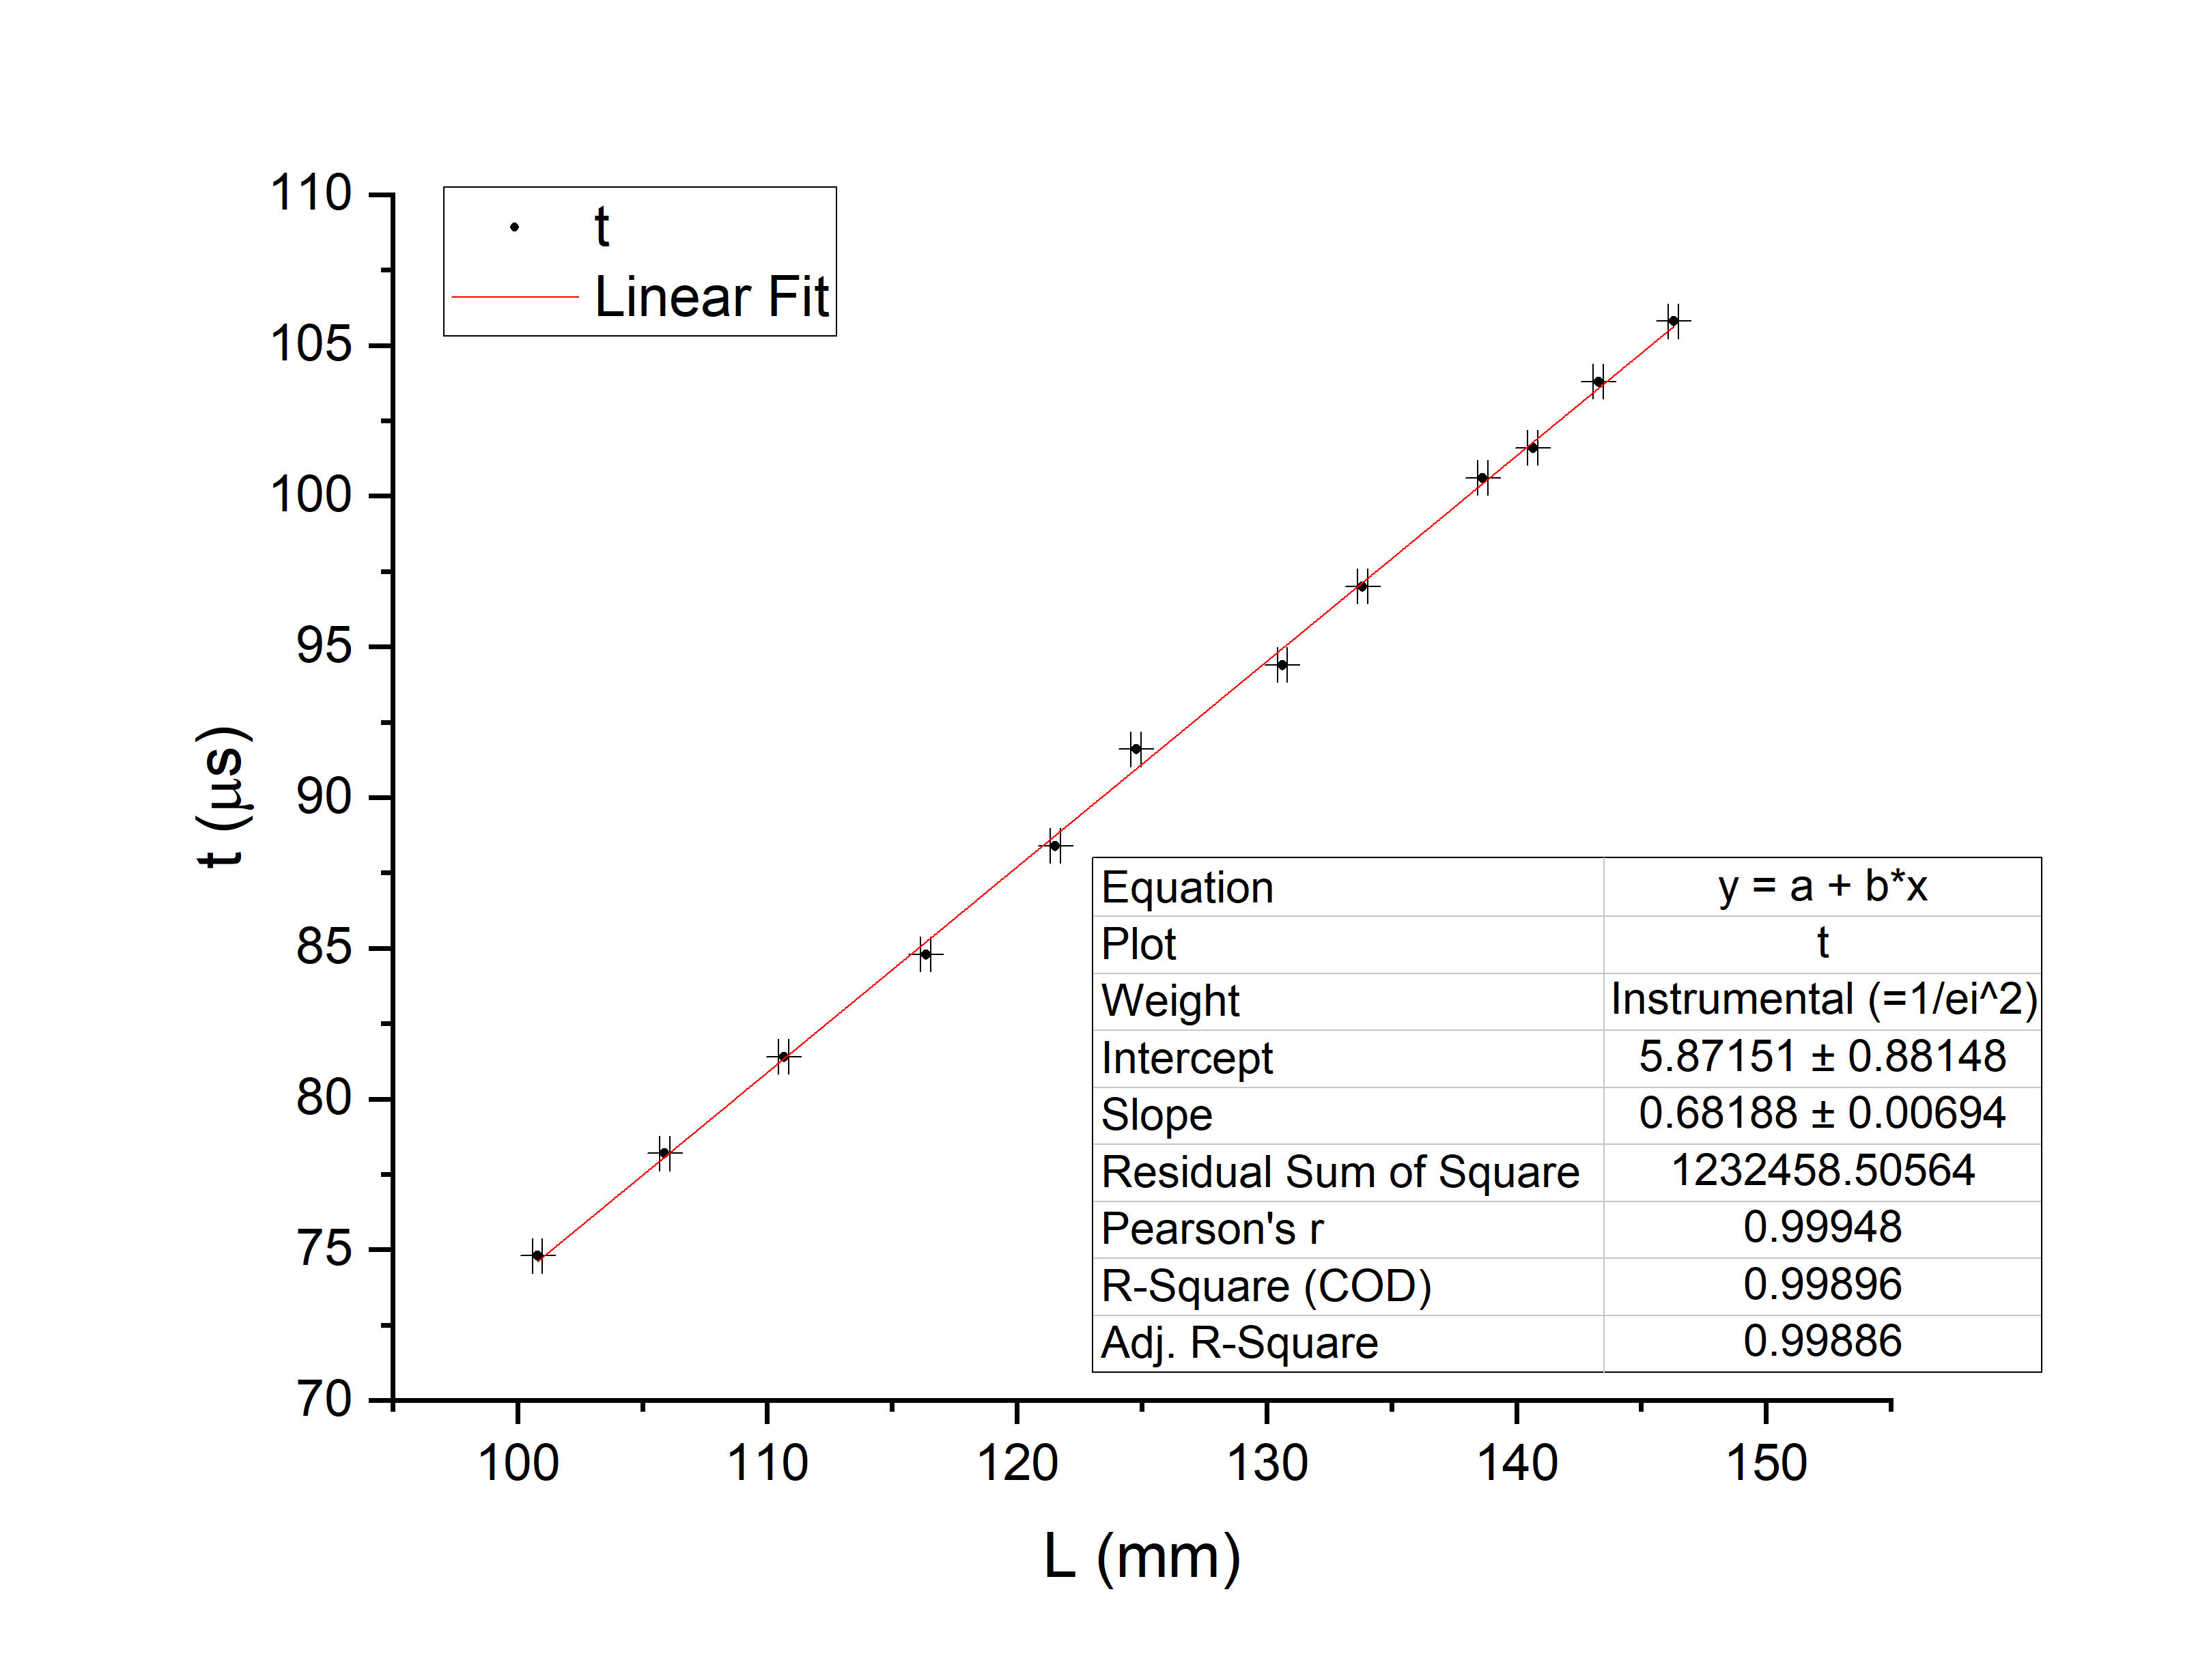
\includegraphics[width=10cm]{method3.png}
    \caption{Linear fit of t v.s. L}
\end{figure} 

\section{Concludsion and Discussion}
\subsection{Conclusion}
In this experiment, we calculate the speed of sound using three methods. Shown below are the experimental results.
\begin{itemize}
    \item From the resonance method: $v_{air}=351.5\pm 1.1m/s$.
    \item From the phase-comparison method: $v_{air}=349.6\pm 0.7m/s$.
    \item From the time difference method: $v_{water}=147\times 10^1\pm 3\times 10^1 m/s$.
\end{itemize} \par 
Judging from the uncertainty, the phase-comparison method provides a more accurate result. According to textbook, the speed of sound in air at 20\textcelsius=344m/s, and the speed of sound in water at 20\textcelsius=1482m/s. Our results in the water are all larger than theory, which is reasonable because in both gas and liquid, the higher the temperature, the larger the speed of sound. But our data still have errors, which will be discussed in 6.2. But for the velocity in the water, it's smaller than the theoratical value. The reasons are discussed in 6.2.

\subsection{Error Analysis}
\begin{itemize}
    \item In resonance method, there exist errors in the measurement of L. It is hard to control when to read the readings because we have to take the readings at the exact moment that the amplitude of the V function starts to decrease. There are too many objective judgements in this step.
    \item In phase-comparison method, we also need to judge when the figure is a straight line by ourselves. Since the figure is changing slightly all the time, the readings are inaccurate.
    \item In time difference method, due to the use of devices, the temperature of water might increase, which results in change of speed of sound in water.
    \item There are too many factors that will disturb the sound wave. And the medium is not 100\% pure. The shown figure on the oscilloscope might not be the actual one.
    \item The wave will lose energy when propagating from S1 to S2, so S2 might receive a different wave from the one that S1 emits.
\end{itemize}	

\subsection{Discussion}
The temperature T must be measured because it is a factor which affects the speed of sound. Take liquid for example, $v=\sqrt{\frac{B}{\rho}}$, where $B$ is the bulk modulus of fluid and $\rho$ is the fluid density, and of course the density is subject to temperature.\par 
In phase-comparison method, we should use ‘straight line’ Lissajous figures as reference because it is the easiest to judge when the same line appears again. For other elliptical figures, it is hard to find out the exact same pattern as the previous time.\par 
In time difference method, we should set the initial distance to be larger than 100mm. Since the speed of sound in water is expected to be around 1500m/s, the time needed for sound to propagate 100mm is $6.67×10^{-5}$s. If the distance is too small, the device is not precise enough to measure the time interval.\par 
We have to measure the speed of sound under the resonance frequency. Only under this circumstance can a standing wave be formed so that the transducer can receive the strongest voltage signal and has the highest sensitivity.

\subsection{Improvement}
\begin{itemize}
    \item Let the machine detect the distance where V reaches its maximum rather than humans.
    \item Do more experiments, apply more linear fits and take the average value as the speed of sound.
    \item Use ultrasonic wave of different frequencies in the resonance frequency range.
\end{itemize}

\newpage
{\LARGE\textbf{APPENDIX}}
\setcounter{section}{0}
\renewcommand\thesection{\Alph{section}}

\section{Measurement Uncertainty Analysis}
\subsection{Apparatus Uncertainty}
\begin{table}[H]
    \centering
    \begin{tabular}{|c|c|}
        \hline
        Apparatus & Type-B Uncertainty\\
        \hline
        Thermometer & $\pm$1\textcelsius\\  
        \hline
        Signal generator & $\pm$ 0.001kHz\\
        \hline
        Scale on the transducer	& $\pm$ 0.001mm\\
        \hline
        Cursor function & $\pm$0.2$\mu s$ \\
        \hline
    \end{tabular}
    \caption{Apparatus Uncertainty}
\end{table}

\subsection{Uncertainty in Analysis of the Resonance Method}
\subsubsection{Uncertainty of $\lambda$}
The slope k is $\frac{\lambda}{2}=4.558\pm 0.015mm$
$$\lambda=2k$$
$$\sigma_\lambda=2\sigma_k=2\times0.014mm=3\times 10^{-5}m$$

\subsubsection{Uncertainty of v}
$$v=\lambda f$$
$$\frac{\partial v}{\partial \lambda}=f=38561Hz$$
$$\frac{\partial v}{\partial f}=9.12\times 10^{-3}m$$
$$\sigma_v=\sqrt{(\frac{\partial v}{\partial \lambda})^2{\sigma_\lambda}^2+(\frac{\partial v}{\partial f})^2{\sigma_f}^2}=\sqrt{38561^2\times(0.03\times10^{-3})^2+(9.12\times 10^{-3})^2\times 1^2}=1.1m/s$$

\subsection{Uncertainty in Analysis of the Phase-comparison Method}
\subsubsection{Uncertainty of $\lambda$}
From 5.3 we can obtain that, $\lambda=9.066\times 10^{-3}\pm 0.019\times 10^{-3}m$
$$\sigma_\lambda=1.9\times 10^{-5}m$$

\subsubsection{Uncertainty of v}
$$v=\lambda f$$
$$\frac{\partial v}{\partial \lambda}=f=38561Hz$$
$$\frac{\partial v}{\partial f}=9.066\times 10^{-3}m$$
$$\sigma_v=\sqrt{(\frac{\partial v}{\partial \lambda})^2{\sigma_\lambda}^2+(\frac{\partial v}{\partial f})^2{\sigma_f}^2}=\sqrt{38561^2\times(1.9\times10^{-5})^2+(9.066\times 10^{-3})^2\times 1^2}=0.7m/s$$

\subsection{Uncertainty in Analysis of the Time Difference Method}
$$\frac{1}{v}=6.82\times 10^{-4}\pm 0.15\times 10^{-4}s/m$$
$$\frac{\partial\frac{1}{v}}{\partial v}=-\frac{1}{v^2}$$
$$\sigma_u=\sqrt{(\frac{\partial\frac{1}{v}}{\partial v})^2{{\sigma_{\frac{1}{v}}}^2}}=\sqrt{(-\frac{1}{(6.82\times 10^{-4})^2})^2\times {0.15\times 10^{-4}}^2}=3\times 10^1m/s$$

\section{Measurement Data}
\begin{table}[H]
    \centering
    \begin{tabular}{|c|c||c|c||}
        \hline
        \multicolumn{2}{|c||}{$L_i[mm]\pm 0.001[mm]$} & \multicolumn{2}{c||}{$L_i[mm]\pm 0.001[mm]$}\\
        \hline
        1 & 23.278 & 7 & 50.465 \\
        \hline
        2 & 27.834 & 8 & 55.218 \\
        \hline
        3 & 32.339 & 9 & 59.802 \\
        \hline
        4 & 36.962 & 10 & 64.334 \\
        \hline
        5 & 41.395 & 11 & 68.886 \\
        \hline
        6 & 46.034 & 12 & 73.271 \\
        \hline
    \end{tabular}
    \caption{Data table for the resonance method}
\end{table}

\begin{table}[H]
    \centering
    \begin{tabular}{|c|c||c|c||}
        \hline
        \multicolumn{2}{|c||}{$L_i[mm]\pm 0.001[mm]$} & \multicolumn{2}{c||}{$L_i[mm]\pm 0.001[mm]$}\\
        \hline
        1 & 23.189 & 7 & 77.526 \\
        \hline
        2 & 32.287 & 8 & 86.587 \\
        \hline
        3 & 41.353 & 9 & 95.945 \\
        \hline
        4 & 50.392 & 10 & 104.934 \\
        \hline
        5 & 59.435 & 11 & 113.834 \\
        \hline
        6 & 68.454 & 12 & 122.790 \\
        \hline
    \end{tabular}
    \caption{Data table for the phase comparison method}
\end{table}

\begin{table}[H]
    \centering
    \begin{tabular}{|c|c|c|}
        \hline
         & $t_i[\mu s]\pm 0.2[\mu_s]$ & $L_i[mm]\pm 0.001[mm]$ \\
        \hline
        1 & 74.8 & 100.806 \\
        \hline
        2 & 78.2 & 105.901 \\
        \hline
        3 & 81.4 & 110.662 \\
        \hline
        4 & 84.8 & 121.534 \\
        \hline
        5 & 91.6 & 124.768 \\
        \hline
        6 & 91.6 & 124.768 \\
        \hline
        7 & 94.4 & 130.630 \\
        \hline
        8 & 97.0 & 133.842 \\
        \hline 
        9 & 100.6 & 138.654 \\
        \hline 
        10 & 101.6 & 140.660 \\
        \hline
        11 & 103.8 & 143.286 \\
        \hline
        12 & 105.8 & 146.286 \\
        \hline
    \end{tabular}
    \caption{Data table for the time difference method(liquid)}
\end{table}

\section{Reference}
\begin{enumerate}[1.]
    \item Young and Freedman. University Physics, Pearson Education Inc., 2019, pp.468-544
    \item Yang Xinyi, Qin Tian, Cao Jianjun, Yi Hankun, Wu Ziyou, Zhang Yifei, Yao Yuan,\\ Mateusz Krzyzosiak, Exercise 4, Measurement of the Speed of Sound
\end{enumerate}

\section{Data Sheet}

\end{document}